\documentclass[12pt, titlepage]{article}

\usepackage{amsmath, mathtools}
\usepackage{fullpage}
\usepackage[round]{natbib}
\usepackage{multirow}
\usepackage{booktabs}
\usepackage{tabularx}
\usepackage{graphicx}
\usepackage{float}
\usepackage{hyperref}
\usepackage{xr}
\externaldocument{../SRS/SRS} 
\hypersetup{
	colorlinks,
	citecolor=black,
	filecolor=black,
	linkcolor=red,
	urlcolor=blue
}
\newcommand{\rref}[1]{R\ref{#1}}
\newcommand{\ddref}[1]{DD\ref{#1}}
%% Comments

\usepackage{color}

\newif\ifcomments\commentstrue

\ifcomments
\newcommand{\authornote}[3]{\textcolor{#1}{[#3 ---#2]}}
\newcommand{\todo}[1]{\textcolor{red}{[TODO: #1]}}
\else
\newcommand{\authornote}[3]{}
\newcommand{\todo}[1]{}
\fi

\newcommand{\wss}[1]{\authornote{blue}{SS}{#1}}
\newcommand{\an}[1]{\authornote{magenta}{Author}{#1}}


\newcounter{acnum}
\newcommand{\actheacnum}{AC\theacnum}
\newcommand{\acref}[1]{AC\ref{#1}}

\newcounter{ucnum}
\newcommand{\uctheucnum}{UC\theucnum}
\newcommand{\uref}[1]{UC\ref{#1}}

\newcounter{mnum}
\newcommand{\mthemnum}{M\themnum}
\newcommand{\mref}[1]{M\ref{#1}}

\begin{document}
	
	\title{Installation Guide: Breaking Effect} 
	\author{Marshall Xiaoye Ma}
	\date{\today}
	
	\maketitle
	
	\pagenumbering{roman}
	
	\section{Revision History}
	
	\begin{tabularx}{\textwidth}{p{3cm}p{2cm}X}
		\toprule {\bf Date} & {\bf Version} & {\bf Notes}\\
		\midrule
		2017-12-13 & 1.0 & New document\\
		\bottomrule
	\end{tabularx}
	
	\newpage
	
	\tableofcontents
	
	\listoftables
	
	\listoffigures
	
	\newpage
	
	\pagenumbering{arabic}
	
	\section{Introduction}
	This document gives a guide to show how to use BreakingEffect step by step with figures. BreakingEffect must be used on Unity3D platform so that it is assumed user has Unity3D installed on device. How to install Unity3D is not covered in this document. Please refer to official Unity manual at \url{https://docs.unity3d.com/Manual/index.html}. \\
	
	Target object of BreakingEffect must be an object containing several child objects. All child objects are considered as pieces after object breaking. BreakingEffect can be used on any 3D model that supported by Unity3D including external object such as .obj model imported from 3DMAX.
	\section{Import entire project and test cases} \label{SecProject}	
	
	\subsection{Import resource unity package}
	
	\begin{enumerate}
		
		\item {Import package following figure one below:}
		Assets $\to$ Import Package $\to$ Custom Package...
		
		\begin{figure}[H]
			\centering
			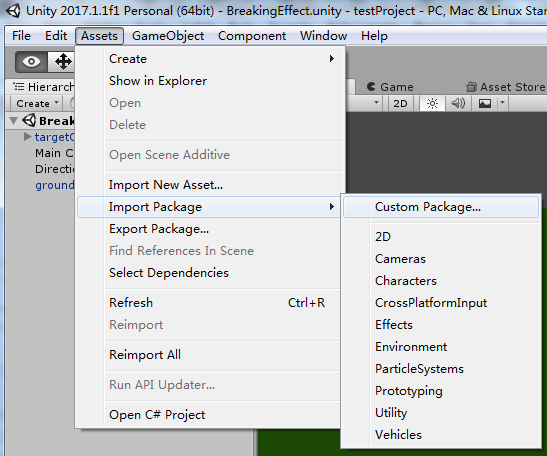
\includegraphics[width=0.7\textwidth]{./Import_package1.png}
			\caption{Import package}
			\label{FigIP}
		\end{figure}
		
		Import unity package /src/BreakingEffect.unitypackage. This package contains all source codes, test codes, scene and unity3d objects for testing demo. Select all items to import.
		After import the package successfully, there will be a scene containing a cube and ground with green texture. 
		
		\item {Scripts}\\
		Source codes and test codes locate at /Assets/script/. 
		
		\begin{figure}[H]
			\centering
			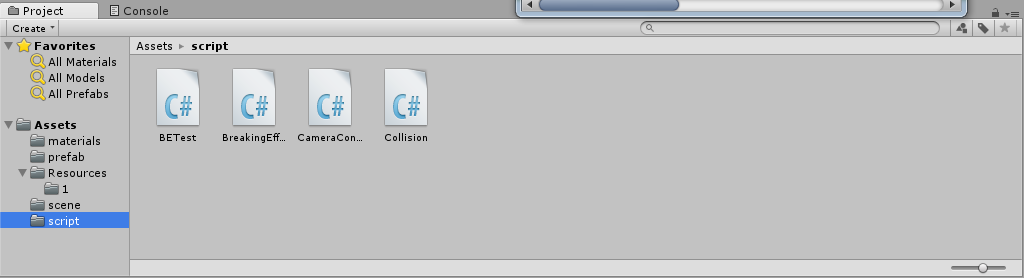
\includegraphics[width=1.1\textwidth]{./script.png}
			\caption{Scripts}
			\label{FigSc}
		\end{figure}
		
		\begin{itemize}		 
		\item BreakingEffect.cs contains codes that implement functional requirements. It needs to be attached to the object where breaking effect happens. 
		\item If a ground in the scene is necessary then the collision.cs must be attached to the ground. 
		\item CameraControl.cs provide free camera controlling. It can be attached to any object in the scene.
		\item BETest.cs contains unit test cases that doesn't need to be attached to any object. Test Runner can be called through Window $\to$ Test Runner that manages all test cases. Name of test functions follows test plan of this project. 
		
		\begin{figure}[H]
			\centering
			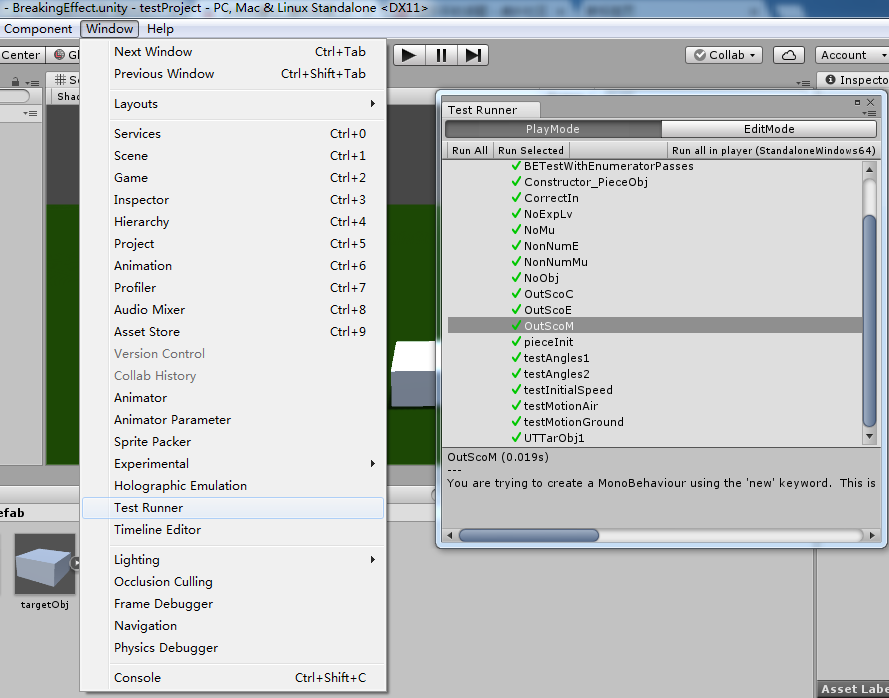
\includegraphics[width=0.8\textwidth]{./testRunner.png}
			\caption{Test Runner}
			\label{FigTR}
		\end{figure}
		
		\end{itemize}
		
		\item {Objects:}\\
		Target objects for testing locate in folder /Assets/prefab. 
		
		\begin{figure}[H]
			\centering
			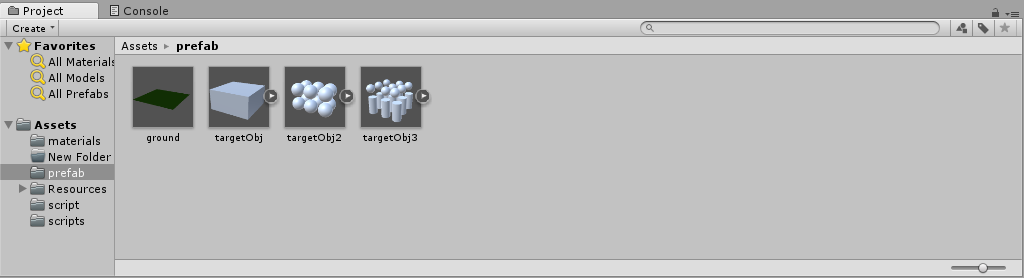
\includegraphics[width=1.1\textwidth]{./prefab.png}
			\caption{Prefab}
			\label{FigPF}
		\end{figure}
	
		targetObj and targetObj2 can be used as target objects in demo to test BreakingEffect. "ground" is default terrain to build a scene with ground. Its texture locates at /Assets/materials.
				
		\item {Left panel:}\\
		On the left panel there should be four objects by default after successful import: targetObj, Main Camera, Directional Light and ground. 
		
		\begin{figure}[H]
			\centering
			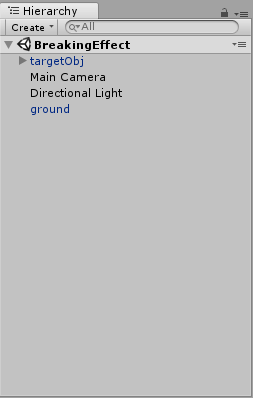
\includegraphics[width=0.5\textwidth]{./Left_Panel.png}
			\caption{Left panel}
			\label{FigLP}
		\end{figure}
		
		For Main Camera and Directional Light please refer to Unity official document:\\ 
		Main Camera: \url{https://docs.unity3d.com/Manual/CamerasOverview.html}\\
		Directional Light: \url{https://docs.unity3d.com/Manual/LightingOverview.html}
		
		\item{View control when running}
		
		Now it is ready to run the demo. Explosion level is 5 and coefficient of ground friction is 0.2 by default. Click play button on the top of Unity3d GUI. Press E button on keyboard to start.\\
		
		\begin{figure}[H]
			\centering
			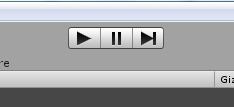
\includegraphics[width=0.5\textwidth]{./play.png}
			\caption{Play}
			\label{FigPlay}
		\end{figure}
		
		Use "w,a,s,d" to move camera.\\
		w: move forward\\
		a: move left\\
		s: move backward\\
		d: move right\\
		Hold mouse left button and space button to rotate on vertical and horizontal direction.
		\item{Add BreakingEffect to any object}\\
		There are some other objects under prefab folder that can be used to play with BreakingEffect. You can also create your own object. However BreakingEffect doesn't provide cutting function for the object because there is no open source plug-in on unity3d that can split an object into pieces at run time. BreakingEffect considers all sub objects as pieces. For example, the "targetObj" consists of 32 small cubes that will be considered as 32 pieces in BreakingEffect. So the target object provided by user should also consists of some child objects.
	\end{enumerate}

	\section{Only use BreakingEffect to your object} \label{SecUse}
	\begin{enumerate}
	\item {Create an object as ground:}
	
	Similar with "ground" provided in package. Create a cube and resize it to what you want such as (1000,1,1000). Make sure your ground have BoxCollider (Is Trigger must be checked) and Mesh Renderer components.Drag /Assets/script/Collision.cs to ground so that it has the Collision (Script) component.
	
	\begin{figure}[H]
		\centering
		\includegraphics[width=0.5\textwidth]{./Ground.png}
		\caption{Ground}
		\label{FigGround}
	\end{figure}
	
	\item {Create your own target object in scene:}\\
	Drag it to left panel, resize and relocate it to where you want.\\
	Drag /Assets/script/BreakingEffect.cs to the target object. Then you target object has a new component on the right panel. Make sure you input E and InputMu here.
	
	\begin{figure}[H]
		\centering
		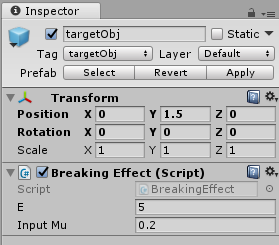
\includegraphics[width=0.5\textwidth]{./input.png}
		\caption{Input}
		\label{FigIn}
	\end{figure}
	
	\item {(Optional)Free camera control:}
	
	Drag /Assets/script/CameraControl.cs to any object in the scene to active free camera controlling when the program running.\\
	\end{enumerate}
\end{document}
